\documentclass[12pt,a4paper,oneside]{article}
\usepackage{ctex,graphicx,setspace,float,fancyhdr,listings,xcolor}
\setstretch{1.25}

% 设置页眉和页脚
\pagestyle{fancy}
\fancyhf{}
\fancyhead[C]{\small 机器学习实验报告} % 中间页眉
\fancyfoot[C]{\small \thepage} % 中间页脚

% 设置代码高亮样式
\lstset{
    language=Python,
    basicstyle=\ttfamily\small,
    numbers=left,
    numberstyle=\tiny,
    stepnumber=1,
    numbersep=5pt,
    showspaces=false,
    showstringspaces=false,
    showtabs=false,
    frame=lines,
    tabsize=4,
    captionpos=b,
    breaklines=true,
    breakatwhitespace=false,
    title=\lstname,
    keywordstyle=\color{blue},
    commentstyle=\color{purple},
    stringstyle=\color{red},
}

\title{
    \vspace*{-2cm} % 调整垂直间距,使图像顶格显示
    
\includegraphics[width=0.8\textwidth]{SYSULogo.pdf} \\[1em]
    \vfill % 添加弹性空间,使内容居中
    \LARGE \textbf{机器学习实验报告2} \\[1em]
    \Large
    \begin{tabular}{rl}
        \textbf{姓名:} & \textbf{陈海弘} \\
        \textbf{学号:} & \textbf{23354049}
    \end{tabular}
    \vfill % 添加弹性空间,使内容居中
}
\date{\Large 2024.10.25}

\begin{document}

\maketitle

\newpage
\tableofcontents
\newpage

\section{作业}
\subsection{pandas库的read\_csv()函数学习}

使用pandas库的read\_csv()函数将训练数据集'train.csv'和测试数据集'test.csv'载入到Dataframe对象中。

首先引入pandas、numpy、matplotlib.pyplot库,然后使用read\_csv()函数读取数据集,将数据集存储到Dataframe对象中。
分别把Datafram中的对象x和y提取出来,用train[ ].values。

使用函数np.array()将Dataframe对象x、y转换为numpy数组。打印查看提取是否正确。

\subsection{一元线性回归模型}
\subsubsection{最小二乘法}
对w和b分别求导后,令导数为0,解出w和b的值。我对w和b的表达式进行了化简,得到了更简洁的表达式。
\begin{equation}
    w = \frac{N \sum_{i=1}^{N} x_i y_i - \sum_{i=1}^{N} x_i \sum_{i=1}^{N} y_i}{N \sum_{i=1}^{N} x_i^2 - (\sum_{i=1}^{N} x_i)^2}
\end{equation}
\begin{equation}
    b = \frac{1}{N} \left( \sum_{i=1}^{N} y_i - wx_i \right)
\end{equation}

重点是在python中公式实现,对np.sum的熟悉运用,我在这里定义了linear\_regression\_params(x, y)函数,再调用前面的arrx,arry。
\begin{lstlisting}
def linear_regression_params(x, y):
    N = len(x)
    w_numerator = N * np.sum(x * y) - np.sum(x) * np.sum(y)
    w_denominator = N * np.sum(x**2) - np.sum(x)**2
    w = w_numerator / w_denominator
    b = (np.sum(y-w*x)) / N
    return w, b
w, b = linear_regression_params(arrx, arry)
    \end{lstlisting}
计算结果:
\begin{figure}[H]
    \centering
    \begin{minipage}[b]{0.3\textwidth}
        \centering
        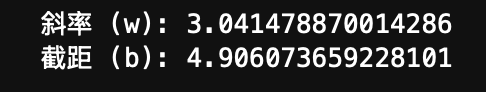
\includegraphics[width=\textwidth]{1}
        \caption{way 1}
        \label{fig:code}
    \end{minipage}
\end{figure}
\subsubsection{梯度下降法}
为了手动实现梯度下降法来进行线性回归模型的训练,特别是小批量随机梯度下降(mini-batch SGD),可以按照以下步骤实现该算法。

首先初始化模型的参数  w  和  b ,可以将它们设为随机值或零值。然后在每次迭代中,随机选取一个小批量数据(即一个小子集),或者是全部数据,然后根据该小批量数据计算损失函数的梯度,并更新参数。以线性回归为例,模型为:
\begin{equation}
    \hat{y}_i = w x_i + b
\end{equation}

然后对参数更新:
\begin{equation}
    w = w - \alpha \frac{\partial L}{\partial w}
\end{equation}
\begin{equation}
    b = b - \alpha \frac{\partial L}{\partial b}
\end{equation}
其中,$\alpha$ 是学习率.

最后是梯度计算,对于线性函数,损失函数的梯度可以写成:
\begin{equation}
    \frac{\partial L}{\partial w} = - \frac{1}{m} \sum_{i=1}^{m} (y_i - \hat{y}_i) x_i
\end{equation}
\begin{equation}
    \frac{\partial L}{\partial b} = - \frac{1}{m} \sum_{i=1}^{m} (y_i - \hat{y}_i)
\end{equation}

重点仍然是代码的实现,我使用了for循环,sum,randn,permutation,mean实现。定义了
mini\_step\_gradient\_descent(x,y,batch\_size,learning\_rate,epochs)函数实现,
其中,batch是每次选的批量大小,learningrate是学习率,就是每次梯度下降的大小,epoch是迭代的次数。
\begin{lstlisting}
def mini_step_gradient_descent(x,y,batch_size,learning_rate,epochs):
    w = np.random.randn()   # 随机初始化斜率
    b = np.random.randn()   # 随即初始化截距
    N = len(x)  # 样本数量
    for epoch in range(epochs):
        indices = np.random.permutation(N)  # 随机打乱样本
        x_shuffled = x[indices] # 打乱后的样本
        y_shuffled = y[indices]
        for i in range(0,N,batch_size): # 每次取batch_size个样本
            x_batch = x_shuffled[i:i+batch_size]    # 取出batch_size个样本
            y_batch = y_shuffled[i:i+batch_size]
            m = len(x_batch)    
            y_pred = w*x_batch + b  # 预测值
            dw = (-1/m) * np.sum((y_batch - y_pred) * x_batch) # 求梯度
            db = (-1/m) * np.sum(y_batch - y_pred)  
            w = w - learning_rate * dw  # 更新斜率
            b = b - learning_rate * db  # 更新截距
        loss = np.mean((y - (w * x + b))**2)    # 计算损失
        print(f'Epoch{epoch+1}/{epoch},Loss:{loss:.4f},w:{w:.4f},b:{b:.4f}')
    return w,b
\end{lstlisting}
计算结果:
\begin{figure}[H]
    \centering
    \begin{minipage}[b]{0.5\textwidth}
        \centering
        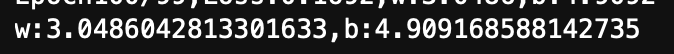
\includegraphics[width=\textwidth]{2}
        \caption{way 2}
        \label{fig:code}
    \end{minipage}
\end{figure}
\subsubsection{矩阵法}
用矩阵表示,假设数据集有 $m$ 个样本,特征有 $n$ 维。$X=\left[ 
\begin{array}{cccc|c} 
    x_{11} & x_{12} & \cdots & x_{1n} & 1 \\
    x_{21} & x_{22} & \cdots & x_{2n} & 1 \\
    \vdots & \vdots & \ddots & \vdots & \vdots \\
    x_{m1} & x_{m2} & \cdots & x_{mn} & 1 
\end{array} \right]$,
实际标签 $Y=\left[ 
\begin{array}{c} 
    y_{1} \\
    y_{2} \\
    \vdots \\
    y_{m}
\end{array} \right]$,
参数 $B=\left[ 
\begin{array}{c} 
    w_{1} \\
    w_{2} \\
    \vdots \\
    w_{n} \\
    b
\end{array} \right]$。

我将使用矩阵表示的解析解来求解线性回归参数  $\theta$ ,其中  $\theta$  包含截距  b  和权重  w 。公式如下:
\begin{equation}
    \theta = (X^T X)^{-1} X^T y
\end{equation}

通过 np.c\_ 将特征矩阵  X  和一个全 1 的列连接起来,表示截距项  b ,然后用 np.linalg.inv 计算矩阵的逆。
np.ones(x.shape[0]) 生成一个全 1 的列向量,然后用 np.c\_ 将其与特征矩阵  x  连接起来,表示截距项  b 。
X.T是X的转置,@是矩阵乘法,np.linalg.inv()是求逆。theta计算得到参数向量,b是theta的第一个元素,w是theta的第二个元素。
\begin{lstlisting}    
def linear_regression_matrix(x,y):
    X = np.c_[np.ones(x.shape[0]),x]
    theta = np.linalg.inv(X.T@X)@X.T@y
    b = theta[0]
    w = theta[1]
    return w,b
\end{lstlisting}
计算结果:
\begin{figure}[H]
    \centering
    \begin{minipage}[b]{0.5\textwidth}
        \centering
        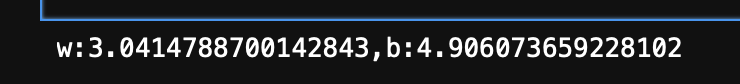
\includegraphics[width=\textwidth]{3}
        \caption{way 3}
        \label{fig:code}
    \end{minipage}
\end{figure}

相比之下,矩阵计算的方法更加简洁,但是在数据量较大时,计算量会增加,因此在数据量较大时,梯度下降法更加适用。
\subsection{测试数据集预测}
使用求解出来的线性回归模型对测试数据集'test.csv'进行预测,输出可视化结果(比如用seaborn或者matplotlib等可视化库来画出测试数据的散点图以及训练好的模型函数图像)。

首先要读取测试数据集,使用模型进行预测,最后可视化结果,用matplotlib库画出散点图和模型函数图像。先画出测试数据的散点图,然后用预测线性回归模型的函数图像画出预测函数,观察预测结果。

scatter()函数用于绘制散点图,plot()函数用于绘制函数图像,show()函数用于显示图像。
具体代码见ipynb文件,下面展示预测结果:
\begin{figure}[H]
    \centering
    \begin{minipage}[b]{0.6\textwidth}
        \centering
        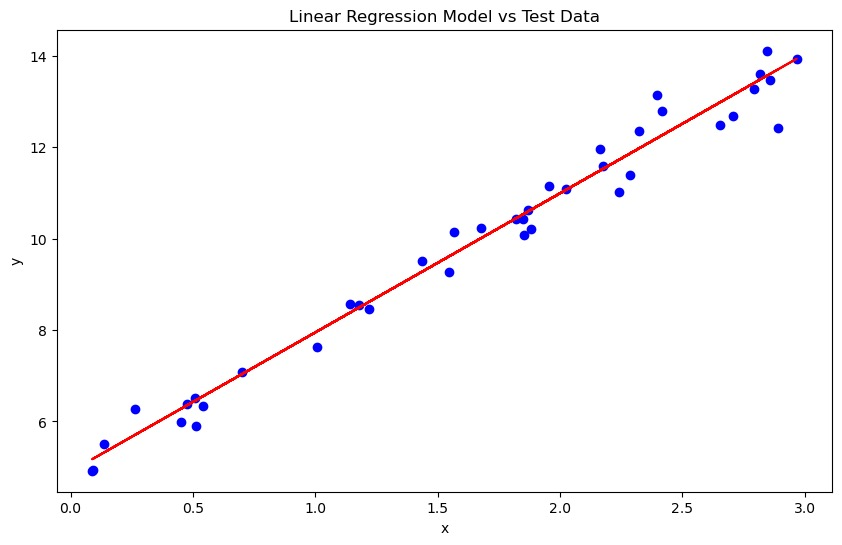
\includegraphics[width=\textwidth]{LR.jpg}
        \caption{Linear Regression Model vs Test Data}
        \label{fig:code}
    \end{minipage}
\end{figure}
看起来预测的还不错,not bad.
\subsection{三元线性回归模型}
训练数据集train2.csv上求一个三元线性回归模型,使得损失函数最小,输出预测结果的均方误差MSE。

有两种方法,第一种就是通过矩阵表示,第二种就是通过梯度下降法。
\subsubsection{矩阵法}
通过矩阵表示的解析解来求解线性回归参数  $\theta$ ,其中  $\theta$  包含截距  b  和权重  w 。和上面提到的类似。
\begin{figure}[H]
    \centering
    \begin{minipage}[b]{0.6\textwidth}
        \centering
        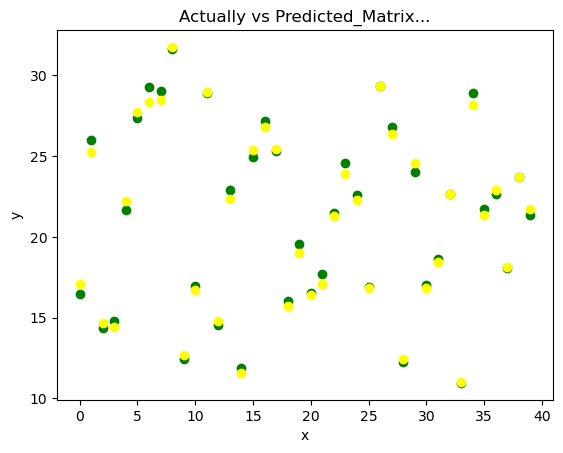
\includegraphics[width=\textwidth]{3M.png}
        \caption{Matrix}
        \label{fig:code}
    \end{minipage}
\end{figure}
\subsubsection{梯度下降法}
我仍然选择用小批量随机下降法,训练数据上优化参数,最终在测试数据上进行预测,计算均方误差MSE。
先定义predeict()函数,用于预测,要熟悉np中常用的函数,如np.dot()是用来计算矩阵乘法的,np.mean()是用来计算均值的,计算均方误差MSE。
np.random.randn是生成随机数,np.random.permutation是生成随机序列,np.sum是求和。

重要代码部分:
\begin{lstlisting}
    for epoch in range(epochs+1):
    shuffled_indices = np.random.permutation(len(x_train))
    x_train_shuffled = x_train[shuffled_indices]
    y_train_shuffled = y_train[shuffled_indices]
    for i in range(0,len(x_train),batch_size):
        x_batch = x_train_shuffled[i:i+batch_size]
        y_batch = y_train_shuffled[i:i+batch_size]
        y_pred_batch = predict(x_batch,w,b)
        dw = -(2/batch_size) * np.dot(x_batch.T,(y_batch-y_pred_batch))
        db = -(2/batch_size) * np.sum(y_batch - y_pred_batch)
        w = w - learning_rate * dw
        b = b - learning_rate * db
\end{lstlisting}

可以看到,两种方法基本上是一致的。
\begin{figure}[H]
    \centering
    \begin{minipage}[b]{0.6\textwidth}
        \centering
        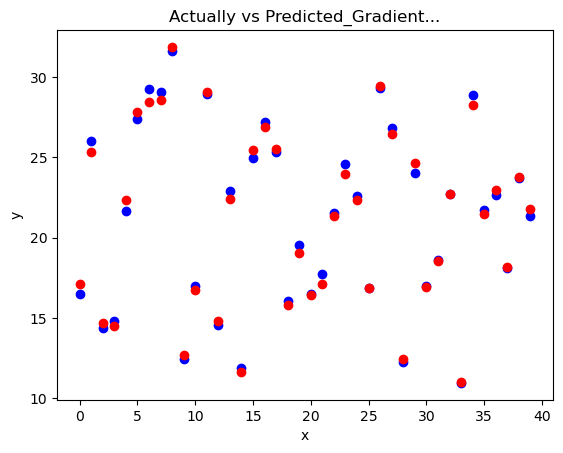
\includegraphics[width=\textwidth]{3G.png}
        \caption{Gradient Descent}
        \label{fig:code}
    \end{minipage}
\end{figure}
\section{总结}
经过这次作业,我对pandas,numpy,matplotlib.pyplot库的使用更加熟练,对于数据的处理和可视化有了更深入的认识。
pd的使用一般在数据处理,对数据的引入。np就更为广泛,array可以取出数据,sum可以求和,mean可以求均值,dot可以求矩阵乘法,random.randn可以生成随机数,random.permutation可以生成随机序列,ones可以生成全1的列向量,c\_可以连接矩阵,linalg.inv可以求逆,.shape可以求矩阵的行列数,T可以求转置,@可以求矩阵乘法。

对plt的使用中,scatter()函数用于绘制散点图,plot()函数用于绘制函数图像,show()函数用于显示图像,figure()函数用于设置图像大小,title()函数用于设置图像标题,xlabel()和ylabel()函数用于设置坐标轴标签。

对于线性回归模型的求解,有三种方法,最小二乘法,梯度下降法,矩阵法。最小二乘法是通过求导解析解,梯度下降法是通过迭代求解,矩阵法是通过矩阵表示解析解。在数据量较大时,梯度下降法更加适用,而在数据量较小时,矩阵法更加简洁。
\end{document}